\chapter{Dyskusja rezultatów}

\section{Przykładowe wyniki}
Wracając do dziennika zdarzeń, który był w sekcji \ref{sec:event_logs} i dla którego przykładowych modeli obliczono w sekcji \ref{sec:alignment-calculation} model dla tego logu znaleziony przy pomocy tego algorytmu to 
\begin{figure}[!ht]
	\centering{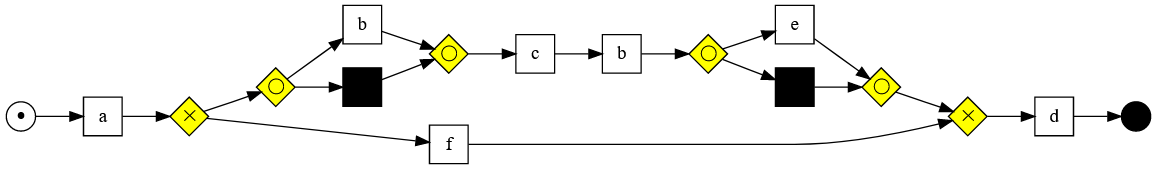
\includegraphics[scale=0.37]{model-example-correct.png}}
	\caption{\label{fig:flow_chart}Znaleziony model}
\end{figure}



Fitness:
0.9550392813257939
Metrics:
Alignment:	1.0
Complexity:	1
Generalization:	0.3426380039733623
Precision:	0.9874986894691236
Simplicity:	0.9230769230769231

Wykres działania w kolejnych generacjach:

\label{alignment-calculation}
Inne przykłady działania to: 

\section{Wyniki w zależności od przyjętych wag poszczególnych metryk}

\subsection{Złożoność}

\section{Wnioski}
